\documentclass[12pt, a4paper]{article}

\usepackage[czech]{babel}
\usepackage{lmodern}
\usepackage[utf8]{inputenc}
\usepackage[T1]{fontenc}
\usepackage{graphicx}
\usepackage{amsmath}
\usepackage[hidelinks,unicode]{hyperref}
\usepackage{float}
\usepackage{listings}
\usepackage{tikz}
\usepackage{xcolor}

\hypersetup{
    colorlinks,
    linkcolor={black!50!black},
    citecolor={blue!50!black},
    urlcolor={blue!80!black}
}
\usepackage[final]{pdfpages}
\usepackage{tabularx}

\definecolor{mauve}{rgb}{0.58,0,0.82}
\usetikzlibrary{shapes,positioning,matrix,arrows}

\newcommand{\img}[1]{(viz obr. \ref{#1})}

\definecolor{pblue}{rgb}{0.13,0.13,1}
\definecolor{pgreen}{rgb}{0,0.5,0}
\definecolor{pred}{rgb}{0.9,0,0}
\definecolor{pgrey}{rgb}{0.46,0.45,0.48}

\usepackage{url}

\usepackage[normalem]{ulem}
\hypersetup{colorlinks,urlcolor=blue}

% hack into hyperref
\makeatletter
\DeclareUrlCommand\ULurl@@{%
  \def\UrlFont{\ttfamily\color{blue}}%
  \def\UrlLeft{\uline\bgroup}%
  \def\UrlRight{\egroup}}
\def\ULurl@#1{\hyper@linkurl{\ULurl@@{#1}}{#1}}
\DeclareRobustCommand*\ULurl{\hyper@normalise\ULurl@}
\makeatother

\lstset{language=Java,
  numbers=left,
  stepnumber=1,
  showspaces=false,
  showtabs=false,
  breaklines=true,
  showstringspaces=false,
  breakatwhitespace=true,
  commentstyle=\color{pgreen},
  keywordstyle=\color{pblue},
  stringstyle=\color{pred},
  basicstyle=\ttfamily\footnotesize,
  moredelim=[il][\textcolor{pgrey}]{$$},
  moredelim=[is][\textcolor{pgrey}]{\%\%}{\%\%}
}


\let\oldsection\section
\renewcommand\section{\clearpage\oldsection}

\begin{document}
	% this has to be placed here, after document has been created
	% \counterwithout{lstlisting}{chapter}
	\renewcommand{\lstlistingname}{Ukázka kódu}
	\renewcommand{\lstlistlistingname}{Seznam ukázek kódu}
    \begin{titlepage}

       \centering

       \vspace*{\baselineskip}

       \begin{figure}[H]
          \centering
          
\includegraphics[width=7cm]{img/fav-logo.jpg}
       \end{figure}

       \vspace*{1\baselineskip}
       {\sc Semestrální práce z předmětu KIV/MBKZ}
       \vspace*{1\baselineskip}

       \vspace{0.75\baselineskip}

       {\LARGE\sc Multiplatformní aplikace zobrazující předpověď počasí\\}

       \vspace{4\baselineskip}
       
		\vspace{0.5\baselineskip}

       
       {\sc\Large Stanislav Král \\}

       \vspace{0.5\baselineskip}

       {A17B0260P}

       \vfill

       {\sc Západočeská univerzita v Plzni\\
       Fakulta aplikovaných věd}


    \end{titlepage}


    \tableofcontents
    \pagebreak

\section{Úvod}

Cílem této práce je vytvoření mobilní multiplatformní aplikace, která bude umožňovat vyhledání a zobrazení předpovědi počasí dle názvu města. Aplikace by měla klást důraz na uživatelsky přívětivý design a implementovat zajímavé animace. Na úvodní obrazovce bude zobrazen seznam předpovědí počasí pro již vyhledané lokace.

   \section{Analýza}

	\subsection{Vývoj multiplatformních aplikaci pomocí frameworku Flutter}
Flutter je open-source framework na jehož vývoji se podílí převážně Google. Cílem Flutteru je nabídnout vývojářům možnost vyvíjet výkonné aplikace, které působí nativně na všech platformách (tzn. že tyto aplikace nelze jednoduše rozeznat od aplikací, jež jsou vyvíjené speciálně na danou platformu). Flutter umožňuje sdílet veškerý kód mezi všemi platformami. Toho je docíleno tak, že knihovna nepoužívá žádné nativní komponenty uživatelského rozhraní dané platformy. Okno aplikace totiž pouze slouží jako plátno a~všechny komponenty si Flutter vykresluje sám. K~vykreslování používá open-source knihovnu Skia, která je napsaná v~jazyce C++, čímž dosahuje plynulosti v zobrazování uživatelského rozhraní. Pro tvorbu aplikací pomocí Flutteru se používá programovací jazyk Dart.

Flutter respektuje rozdíly v~chování uživatelských rozhraní mezi mobilními operačními systémy, čímž pomáhá aplikacím psaným v~tomto frameworku působit tak, jako kdyby byly nativní a~cílené právě pro danou platformu. Mezi hlavní rozdíly mezi platformami, jež tato knihovna implementuje na jednotlivých platformách zvlášt, patří například vertikální rolování obrazovky, ikony nebo typografie.

Při nasazení na platformu Android je C a~C++ kód enginu kompilován pomocí Android NDK (Native Development Kit), zatímco Dart kód se s~využitím kompilace typu ahead-of-time kompiluje do nativních knihoven pro procesory ARM a~x86. Tyto knihovny jsou poté použity ve vygenerované nativní aplikaci, která slouží jako hostitel, a~z~celého projektu je následně vytvořen APK balík. 

Podobně probíhá i~nasazení aplikace na platformu iOS, kdy je kód enginu překládán pomocí LLVM. Kompilace do nativních knihoven znamená, že narozdíl od ostatních frameworků pro tvorbu multiplatformních aplikací, jsou Flutter aplikace zcela nativní. 

Při vyvíjení aplikací pomocí Flutteru je použit virtuální stroj, který umožňuje upravovat zdrojový kód aplikace bez nutnosti ji restartovat. Tato funkce má největší význam při tvorbě uživatelského rozhraní, kdy se jednotlivé změny v~designu aplikace ihned projeví na zařízení. 

\begin{figure}[!ht]
\centering
{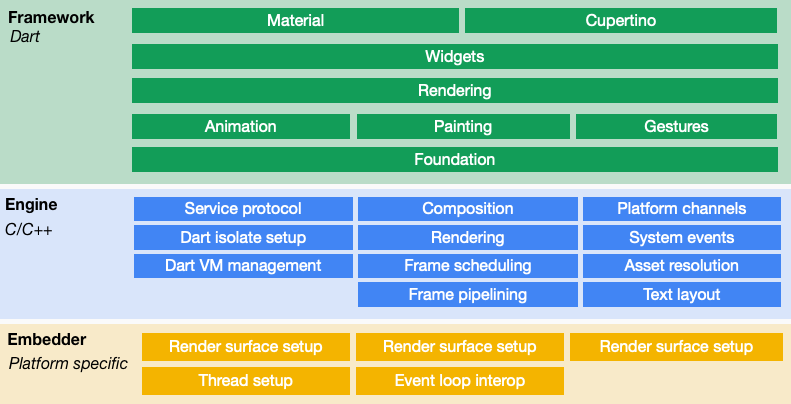
\includegraphics[width=13.5cm]{img/flutter-architecture.png}}
\caption{Diagram architektury Flutter}
\label{fig:flutter-architecture}
\end{figure}

Prvky uživatelského rozhraní, které Flutter nabízí, se snaží co nejvěrněji napodobit ty nativní. Prvky napodobující prvky platformy Android se nachází v~balíku \texttt{Material} a~prvky platformy iOS v~balíku \texttt{Cupertino}. Tým vývojářů Flutteru bere ohledy na aktualizace mobilních operačních systémů a~změny v~uživatelských rozhraní včas implementuje do svého frameworku.

Flutter dále umožňuje psát nativní kód specifický pro danou platformu pomocí konstrukce zvané \texttt{platform channel}, která funguje na principu asynchronního předávání zpráv. Část aplikace Flutter pošle hostitelské nativní aplikaci zprávu, která asynchronně na tuto zprávu odpoví. To umožňuje přístup k~nativnímu API dané platformy. 

Na konci roku 2019, v~každoročním shrnutí služby GitHub, je programovací jazyk Dart, který se v~dnešní době používá nejvíce právě ve Flutter aplikacích, označen jako jazyk s~nejrychleji rostoucím počtem vývojářů, jež ho používají pro vývoj aplikací\footnote{\url{https://octoverse.github.com/#fastest-growing-languages}}.


\subsection{Výběr API pro získání dat předpovědi počasí}

Nutným předpokladem pro efektivní vývoj mobilní aplikace, která zobrazuje předpověď počasí, je správný výběr služby, jež zpřístupňuje API umožňující získávání dat obsahující předpověď počasí dle názvu města v přehledně strukturovaném formátu.


\subsubsection{Služba OpenWeather}

Služba OpenWeather \footnote{OpenWeather - \ULurl{https://openweathermap.org/api}} nabízí pro registrované uživatele tarifní plán zdarma, v rámci kterého lze přistupovat k API této služby, jež poskytuje dle názvu města data obsahující předpověď počasí pro danou oblast. Pro použití tohoto API je však nutné si nechat vygenerovat API klíč, který musí být použit při každém volání tohoto API. Data poskytována tímto API jsou dostupná ve formátu JSON, XML nebo HTML. Tato služba nabízí krátkodobou i dlouhodobou předpověď počasí a plán zdarma je omezen 1000 přístupy k API denně.


\subsubsection{Služba Weatherbit}

Tato služba, jež poskytuje v rámci svého bezplatného tarifního plánu API poskytující předpověď počasí, umožňuje registrovaným uživatelům až 500 přístupů denně k předpovědím zdarma\footnote{Weatherbit - \ULurl{https://www.weatherbit.io/api}}. Toto API je pečlivě popsané a dokonce nabízí k dispozici dokumentaci pomocí služby \textbf{Swagger}.


\subsubsection{Služba MetaWeather}

Služba MetaWeather \footnote{MetaWeather - \ULurl{https://www.metaweather.com/}} slouží jako agregátor dat předpovědi počasí ze služeb \textbf{BBC}, \textbf{Forecast.io},  \textbf{HAMweather} nebo například \textbf{OpenWeather}, čímž slibuje větší přesnost svých předpovědí. API, které tyto agregované předpovědi poskytuje, je dostupné zdarma a bez jakýchkoliv omezení. Uživatel tohoto API je však povinen ve své práci uvést odkaz na webovou stránku této služby a neměl by toto API používat ke komerčním účelům. 

Poskytované API je velmi jednoduché a umožňuje vyhledávat konkrétní předpovědi pro dané lokace pomocí názvu měst. Nevýhodou této služby je to, že počet měst, pro které poskytuje předpověď počasí, je velmi malý. Například v České republice je dostupná předpověď pouze pro hlavní město Praha.


\section{Uživatelské rozhraní vytvořené aplikace}\label{chapt:ui}

Aplikace implementuje vlastní design uživatelského rozhraní, který je identický na obou hlavních mobilních platformách, a tak se přímo neřídí doporučeným designem iOS nebo Android aplikací.

\subsection{Úvodní obrazovka aplikace}

Na úvodní obrazovce aplikace je zobrazen název aplikace a logo frameworku Flutter. Pod těmito komponentami je umístěn seznam měst, ke kterým si uživatel již v minulosti vyhledal předpověd počasí. Pro tato města je automaticky získána aktuální předpověď počasí. Následně se pod tímto seznamem nachází vstupní pole, které slouží pro zadání názvu města, pro něhož si uživatel přeje zjistit předpověď počasí. Tlačítkem, jež je umístěno ve spodní části obrazovky, se spustí vyhledávání předpovědi počasí pro dané město.

\begin{figure}[h]
    \centering
    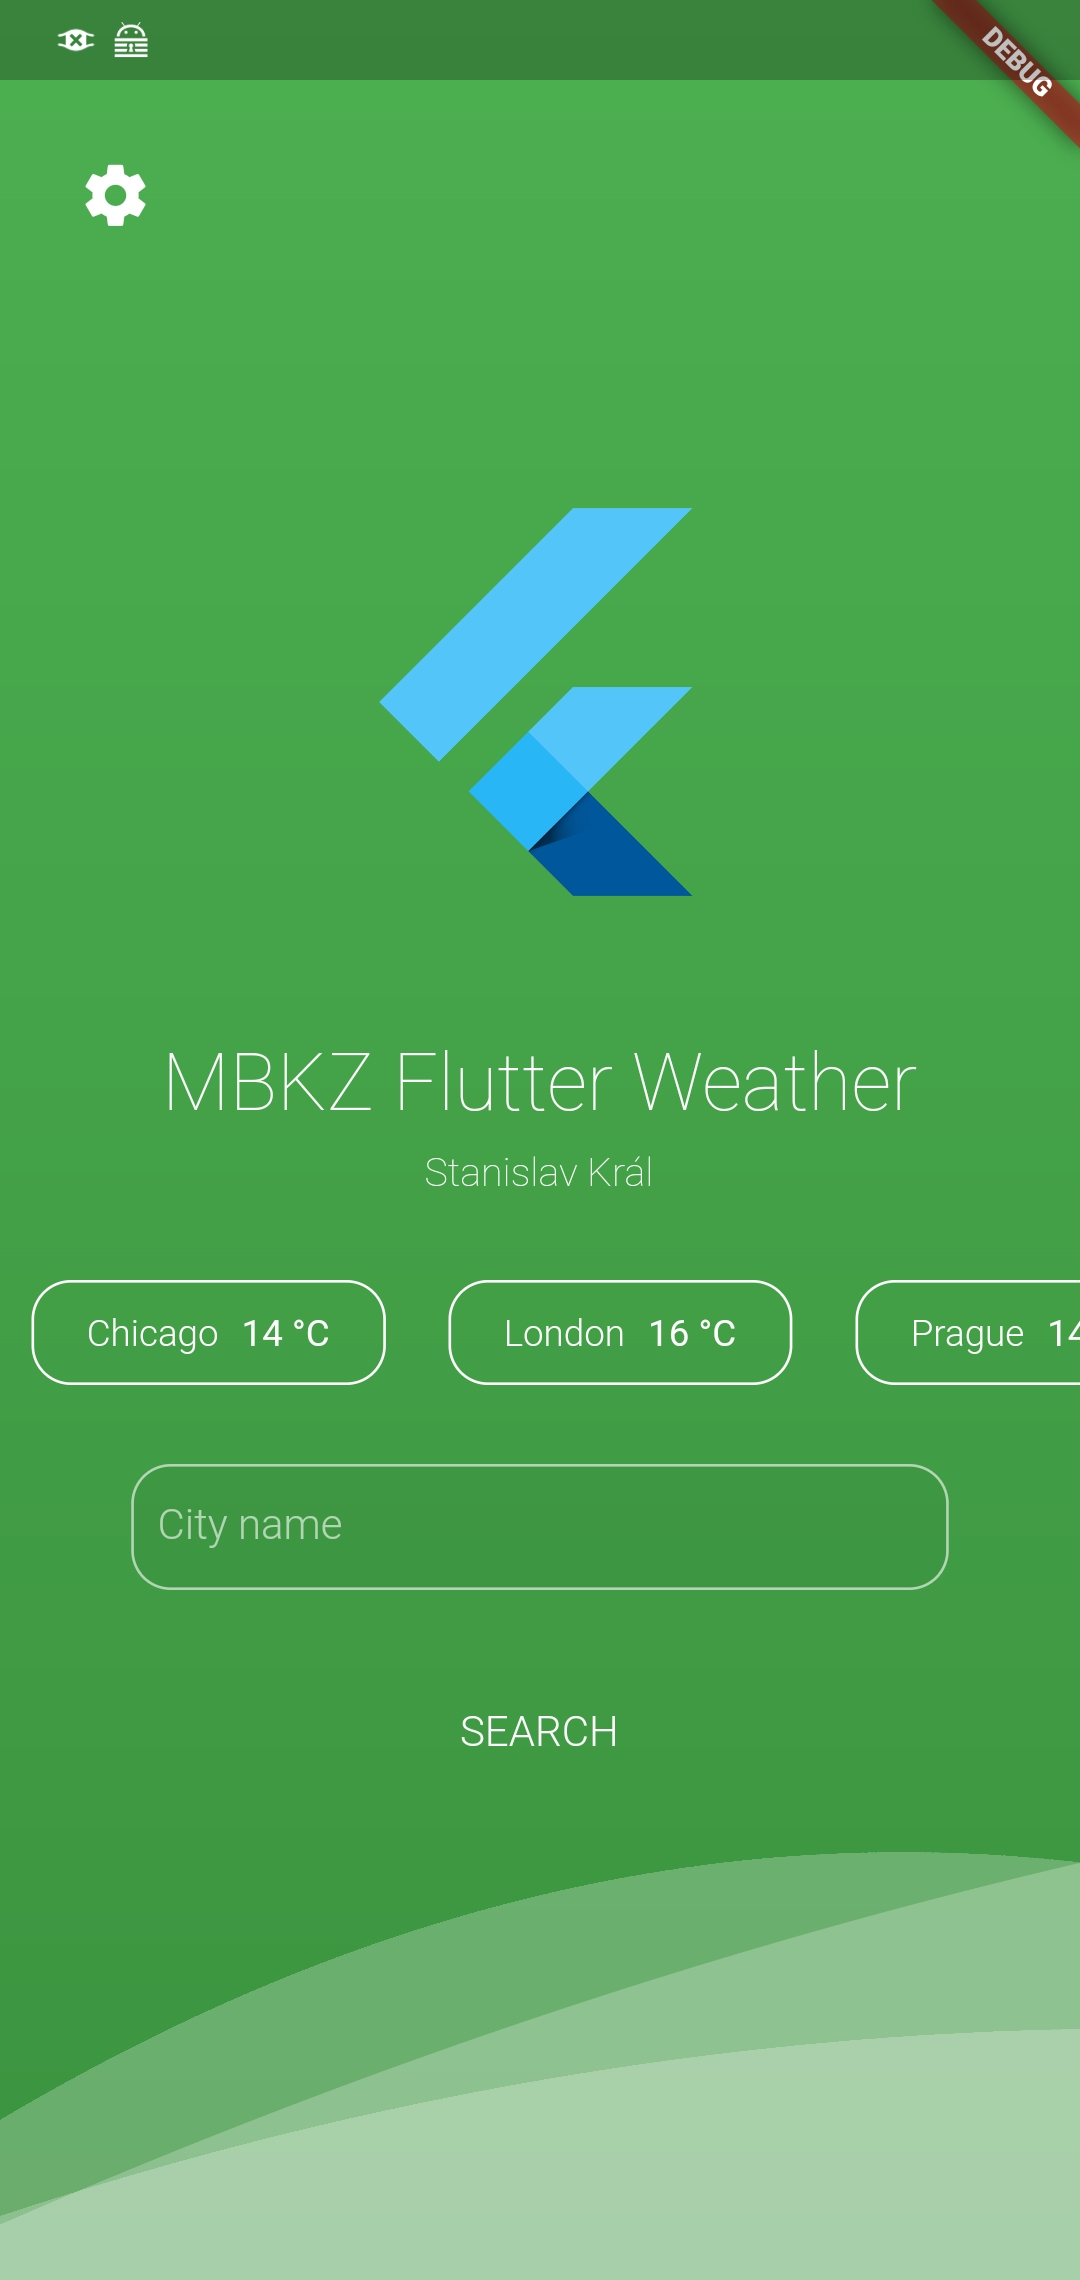
\includegraphics[width=0.40\textwidth]{img/app-menu.jpg}
    \caption{Úvodní obrazovka aplikace}
    \label{fig:mesh1}
\end{figure}

Pokud uživatel klikne na nějakou položku ze seznamu již vyhledaných měst, tak se otevře detailní předpověď pro vybrané město. Dlouhým stisknutím prstu na vybranou položku je tato položka z tohoto seznamu odebrána.

\subsection{Obrazovka předpovědi počasí}

Na této obrazce se nachází název města, ke kterému je aktuálně zobrazována předpověd počasí. Pod názvem města je zobrazené datum, ke kterému se předpověď vztahuje. Předpověď popisuje očekávané počasí za jeden konkrétní den. Uprostřed obrazovky je zobrazena předpovídaná průměrná teplota, minimální teplota a maximální teplota za daný den. Pod teplotami jsou zobrazeny informace o vlhkosti a rychlosti větru.

Horizontálním táhnutím prstu po obrazovce lze přepínat mezi předpověďmi na nadcházející dny (celkem 5 předpovědí). Každý hlavní typ počasí, které v daný den panuje, je reprezentován animovaným pozadím této obrazovky, jež se při změně typu mění a vizualizuje tak například, když má v daný den pršet, sněžit nebo pokud má být jasná obloha.

\begin{figure}[!htb]
\minipage{0.32\textwidth}
  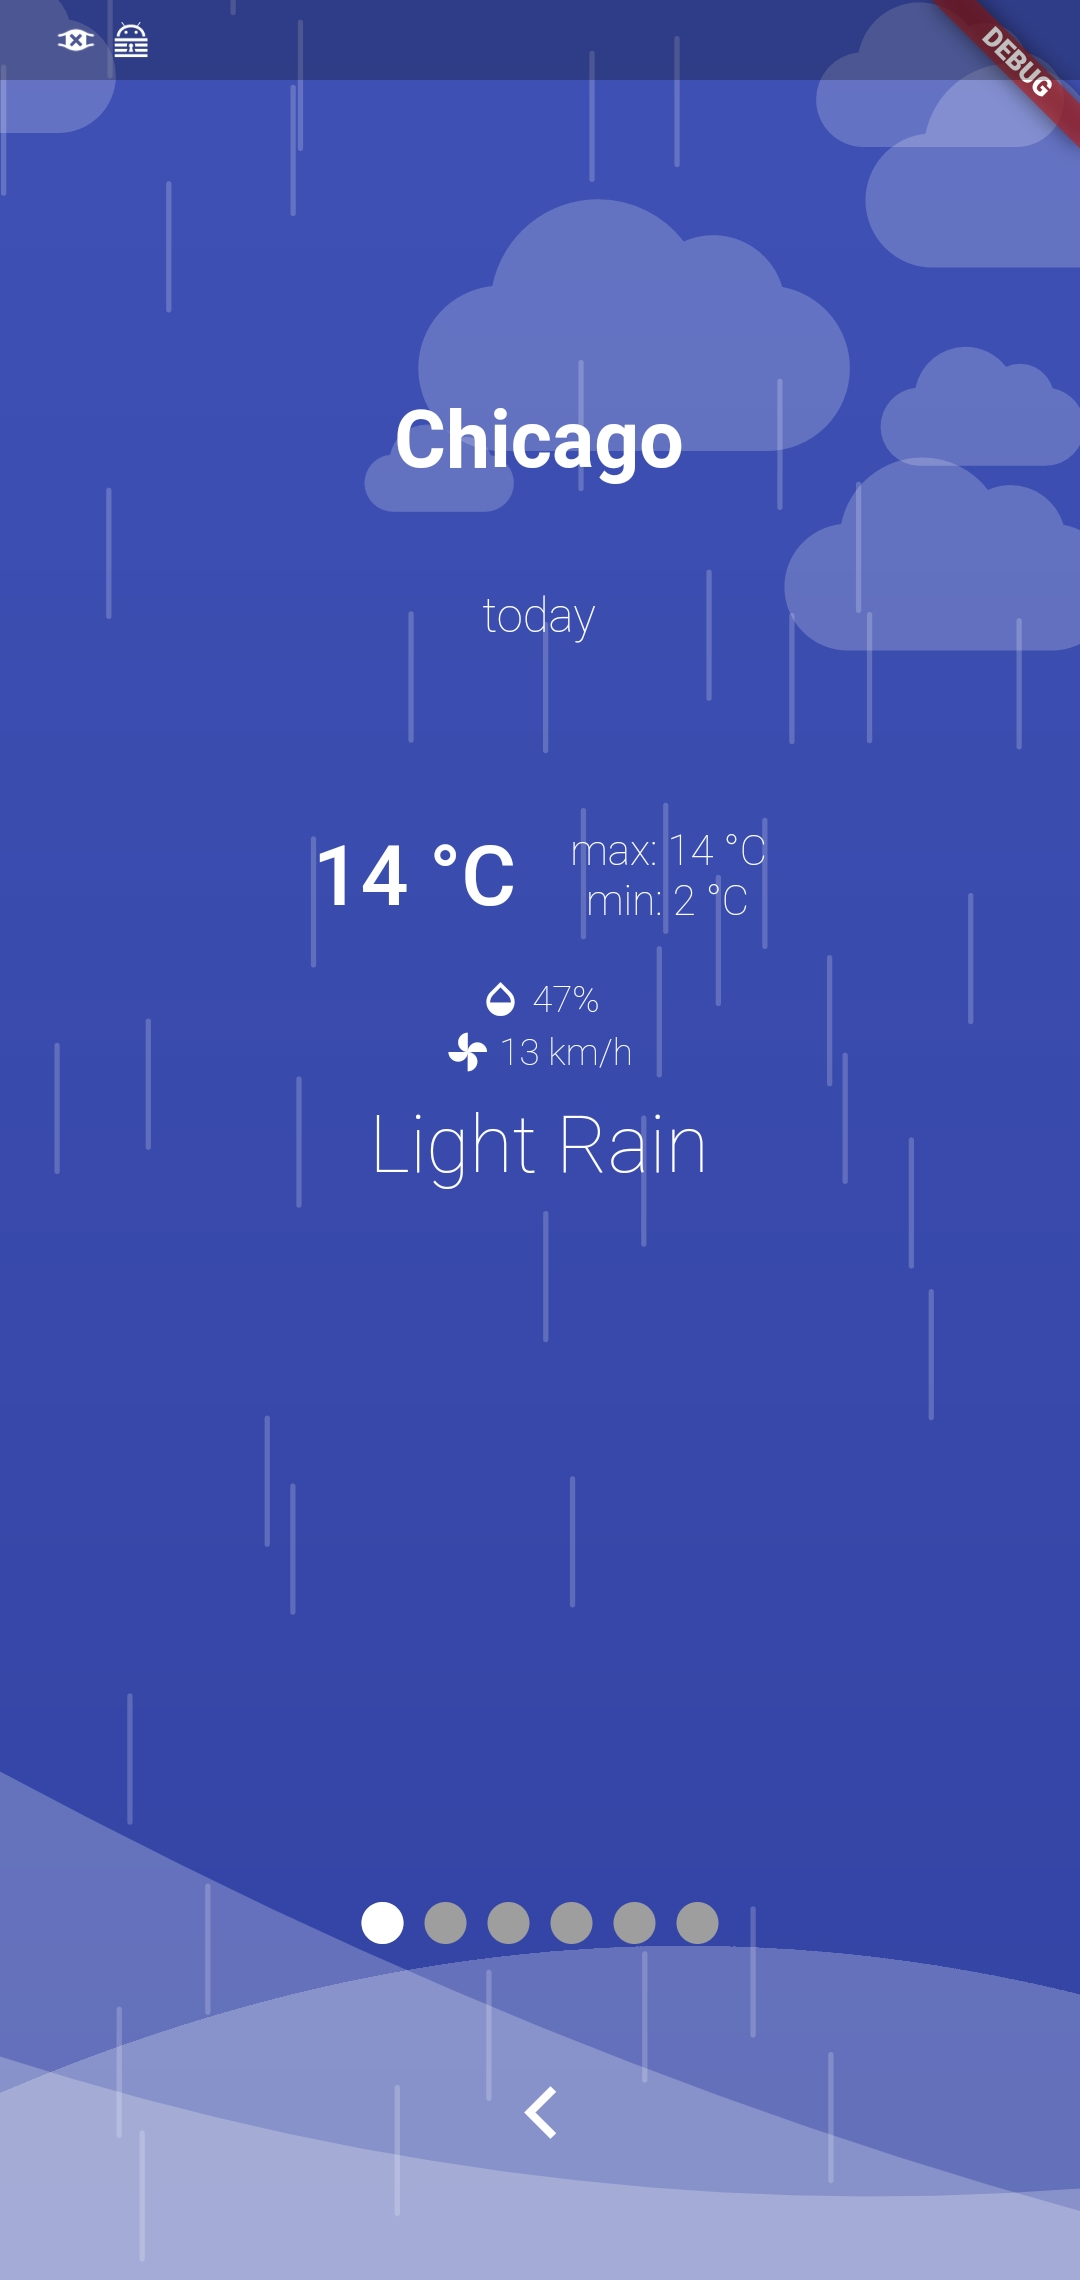
\includegraphics[width=\linewidth]{img/app-rain.jpg}
\endminipage\hfill
\minipage{0.32\textwidth}
  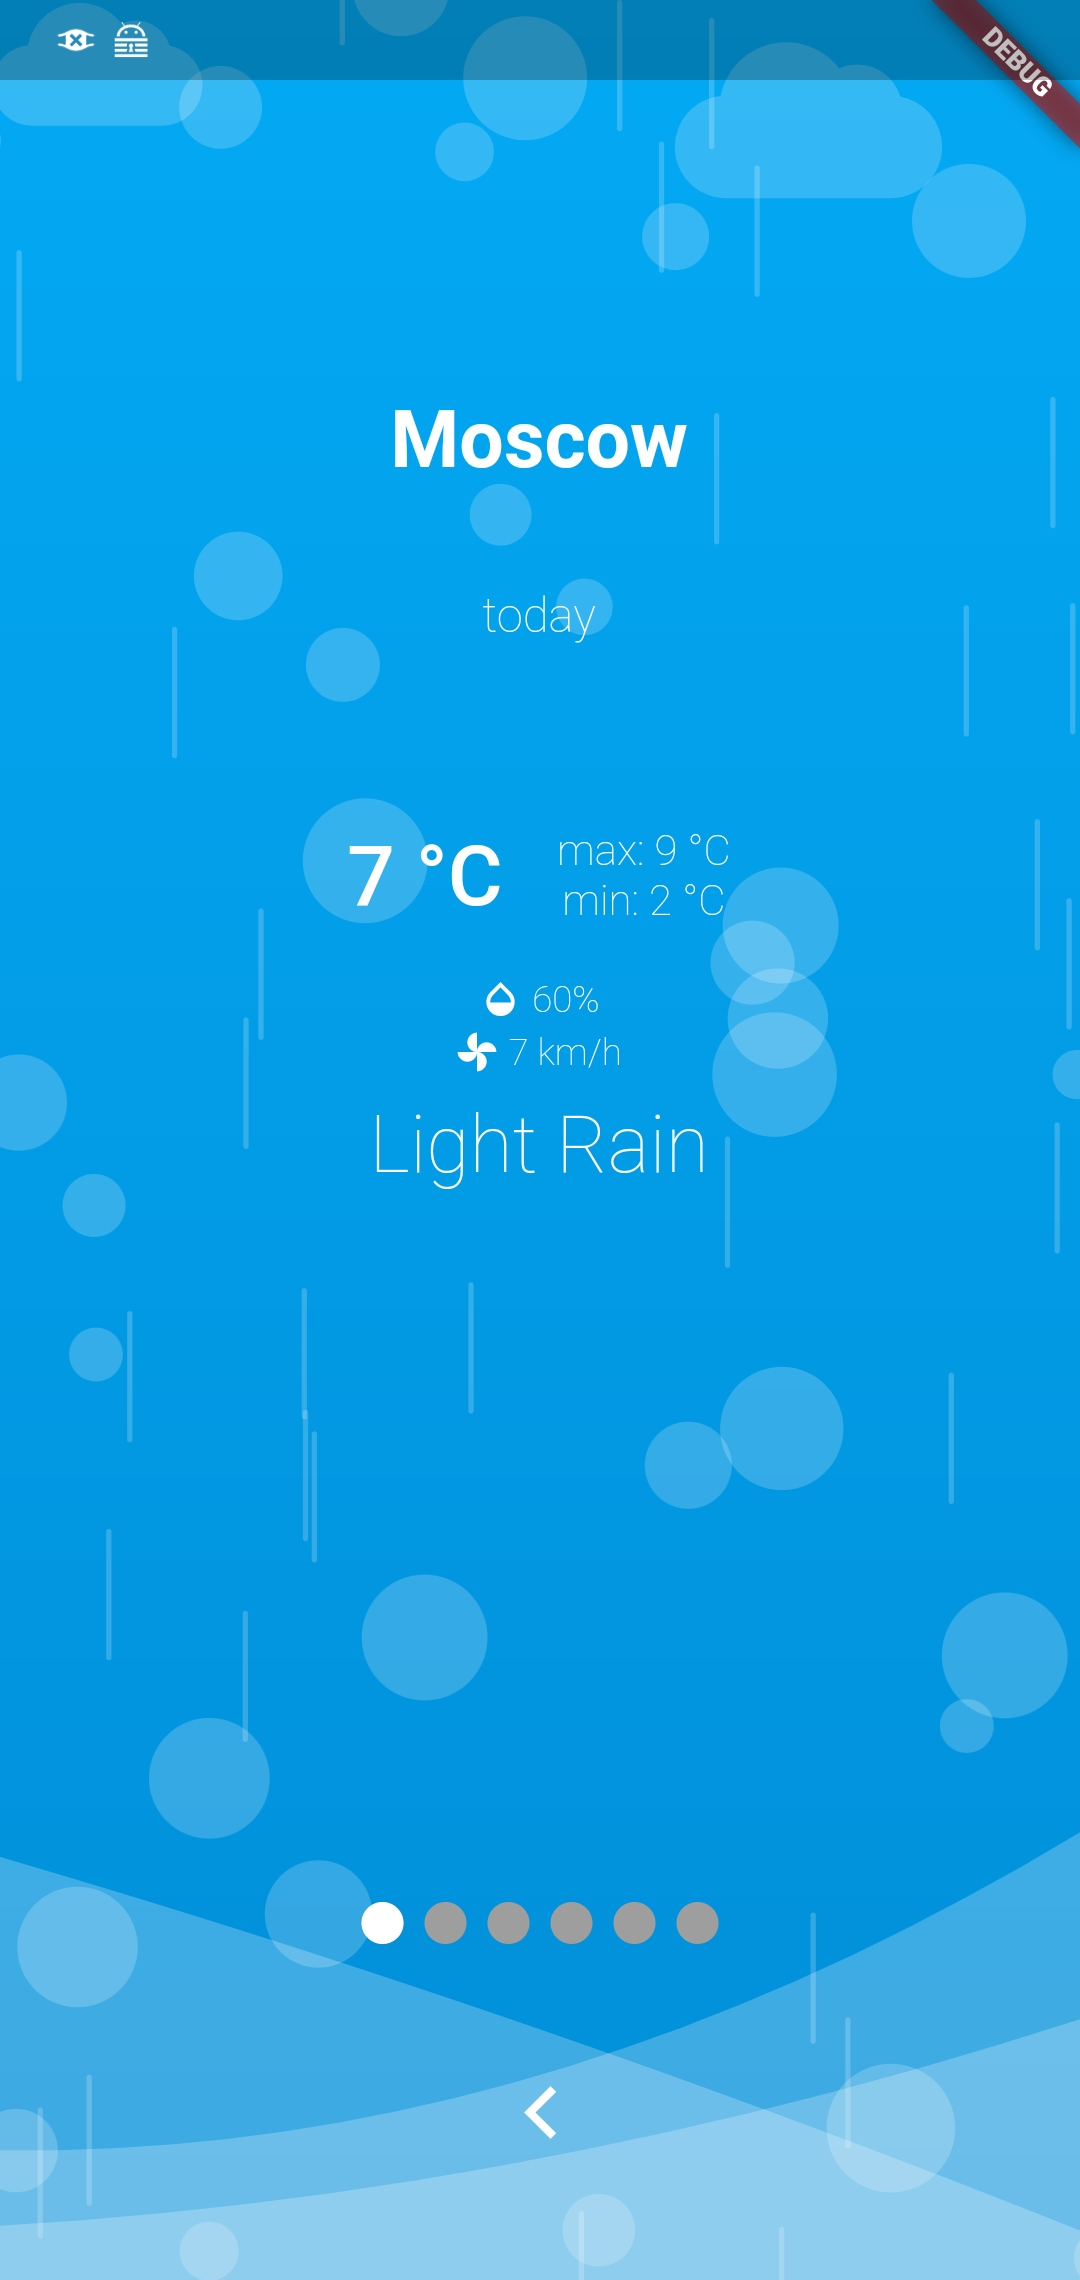
\includegraphics[width=\linewidth]{img/app-sleet.jpg}
\endminipage\hfill
\minipage{0.32\textwidth}%
  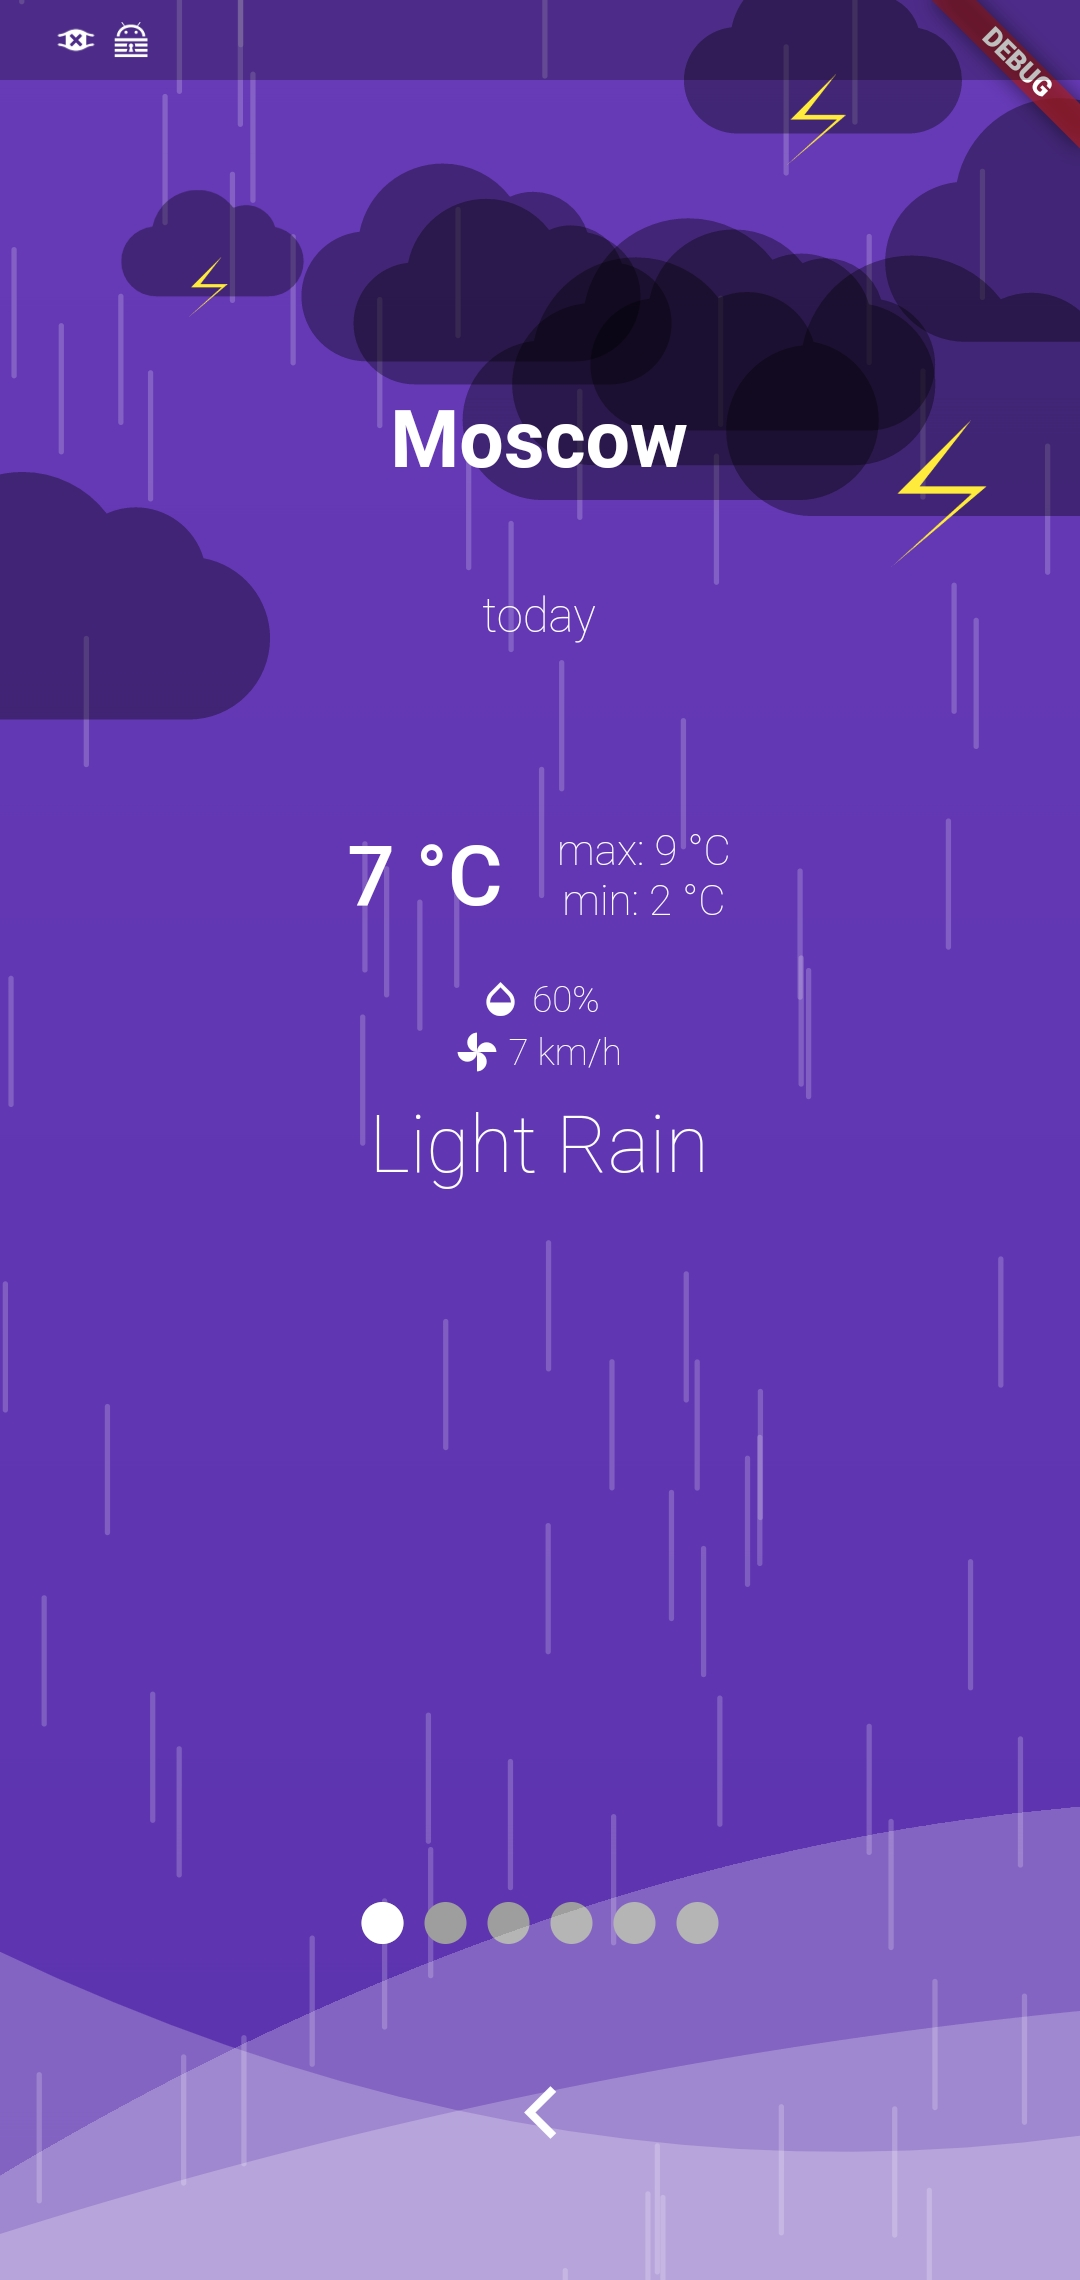
\includegraphics[width=\linewidth]{img/app-thunder.jpg}
\endminipage

  \caption{Ukázka různých typů počasí, jež aplikace vizualizuje.}
\end{figure}

\subsection{Dialog s nastavením aplikace}

V tomto dialogu, jež se otevře po kliknutí na ikonu ozubeného kola umístěného na v levém horním rohu úvodní obrazovky, má uživatel možnost pomocí přepínače přepnout nastavení, jestli se mají v aplikaci používat metrické nebo imperiální jednotky. Tato preference je uložena napříč jednotlivými spuštěními aplikace.

Pod přepínačem metrických a imperiálních jednotek se nachází tlačítko, jež slouží pro vymazání historie jich vyhledaných měst.

\begin{figure}[!ht]
\centering
{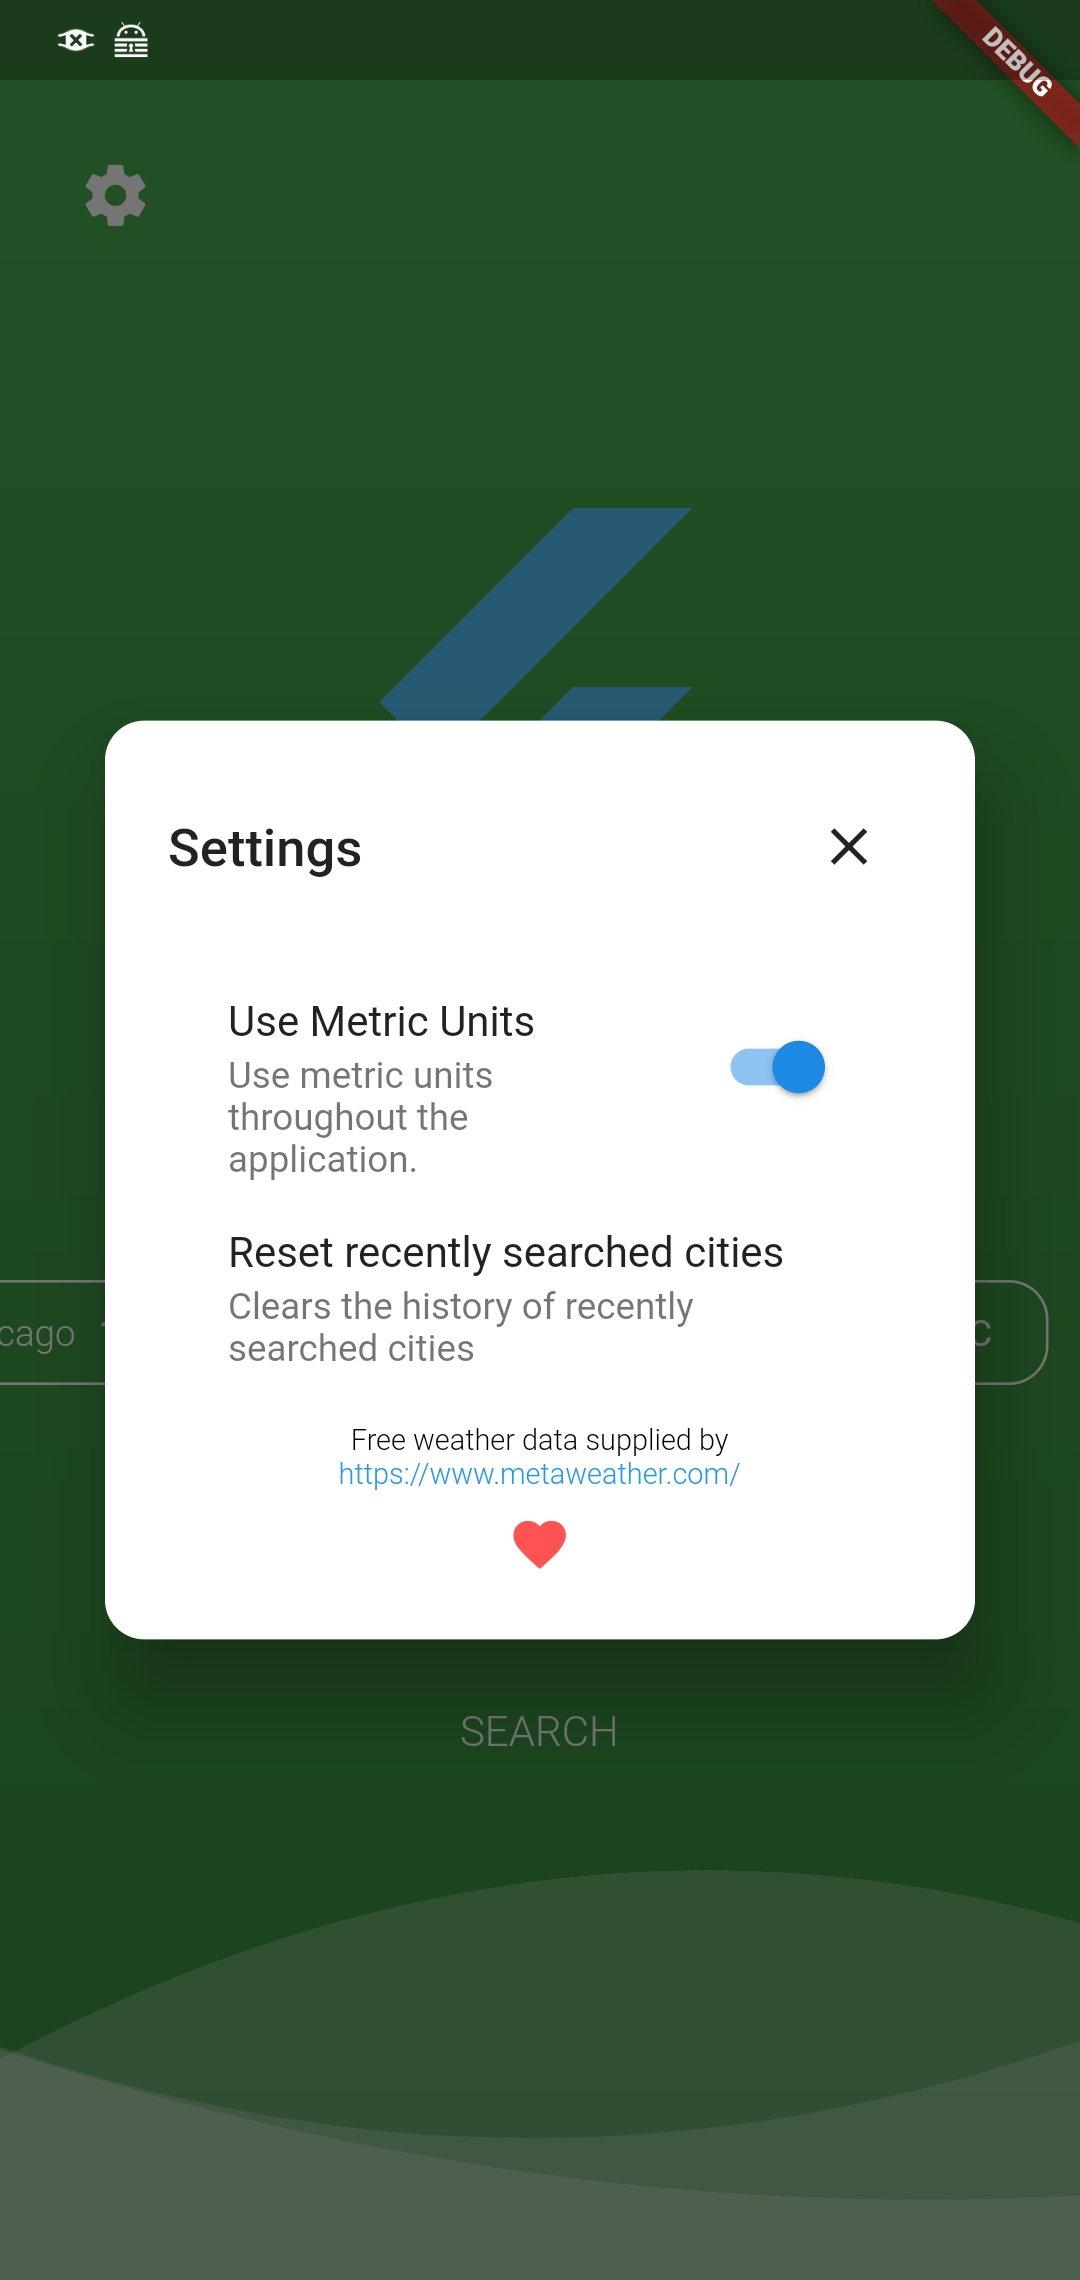
\includegraphics[width=0.40\textwidth]{img/app-settings.jpg}}
\caption{Dialog s nastavením aplikace}
\label{fig:flutter-architecture}
\end{figure}

Kliknutím na odkaz použité služby pro získávání předpovědi počasí je ve výchozím internetovém prohlížeči zařízení otevřena domovská stránka této služby.

\section{Popis implemtance}


\subsection{Správa stavů aplikace}


Při vývoji mobilních aplikací ve frameworku Flutter se často setkáváme s~pojmem \textbf{state management}, jež lze volně přeložit do češtiny jako \textbf{správa stavů aplikace}. Tento pojem se při využití tohoto frameworku používá proto, že na rozdíl od vývoje nativních aplikací se pro tvorbu uživatelského rozhraní v~knihovně Flutter využívá spíše deklarativního paradigmatu, kdy se jasně deklarují jednotlivé stavy, ve kterých se aplikace může nacházet. Základní myšlenku tvorby uživatelského rozhraní v~tomto frameworku představuje následující rovnost:
$$
user\_interface = f(application\_state)
$$

V~praxi to znamená, že v~celém kódu Flutter aplikace například nelze nalézt žádné imperativní volání nastavení textu komponenty pro zobrazení textu na obrazovce, zatím co se například na
 platformě Android v~nativním vývoji pro tuto operaci používá metoda \texttt{setText}. Každá část aplikace může mít vlastní stav, který se v~kódu implementuje tak, že se vytvoří potomek 
třídy \texttt{State} a~nadefinují se jednotlivé atributy tohoto stavu. Při aktualizaci stavu se tato celá část aplikace vykreslí znovu. Tento koncept lze nejlépe pochopit na následující 
ukázce kódu:

\begin{lstlisting}[language=Java,caption={Jednoduchá demonstrace aktualizace uživatelského rozhraní ve frameworku Flutter.},captionpos=b, label={lst:sm-showcase}]
class _MyHomePageState extends State<MyHomePage> {
  int _counter = 0;
  void _incrementCounter() {
    // setState method forces the UI to redraw by
    // saying the state of the screen has changed
    setState(() {
      _counter++;
    });
  }
  @override
  Widget build(context) {
    return Scaffold(
      body: Center(
        child: Text(
          'Counter value: ' + _counter.toString(),
        ),
      ),
      floatingActionButton: FloatingActionButton(
          onPressed: _incrementCounter),);
  }
}
\end{lstlisting}

Avšak při vývoji složitejší aplikace brzy zjistíme, že při definici velké množiny stavů se bez sofistikovanější správy stavů kód aplikace brzy stane nepřehledným. Přístup ukázaný v~ukázce \ref{lst:sm-showcase} slouží jen k~demonstraci konceptu aktualizace uživatelského rozhraní a~nepředstavuje vhodné řešení managementu stavů aplikace. V~praxi se zásadně používají komunitou vytvořené knihovny, mezi které patří například \texttt{provider}, \texttt{MobX}, \texttt{redux} nebo \texttt{flutter\_bloc}. Pro správu stavů obrazovek a~komponent v aplikaci vytvořené v rámci této práce byla zvolena knihovna \texttt{flutter\_bloc}, jež implementuje architekturu \textbf{BloC}.

\subsection{Použitá architektura pro správu stavů}

Ve vytvořené aplikaci je pro správu stavů použita architektura BloC (Bussiness Logic Components), jež rozděluje kód aplikací do tří hlavních částí: 
\begin{itemize}
        \item \textbf{data} -- datová část je zodpovědná za uložení a~manipulaci s~daty aplikace;
        \item \textbf{byznysová logika} -- úkolem této vrstvy je reagovat na události z~prezentační vrstvy novými stavy aplikace;
        \item \textbf{prezentační vrsva} -- uživatelské rozhrání aplikace je vykreslováno na základě získaného stavu z~byznysové logiky.
\end{itemize}

\begin{figure}[!ht]
\centering
{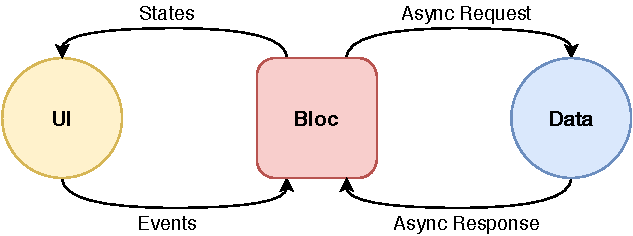
\includegraphics[width=13.5cm]{pdf/bloc-diagram.pdf}}
\caption{Diagram architektury BloC}
\label{fig:vrp-recognition-diagram}
\end{figure}

Obsluha jednotlivých událostí je asynchronní a~prezentační vrstvě může být během jedné obsluhy události předáno několik stavů.


\subsubsection{Management stavů procesu získávání předpovědi počasí}

Pro management stavů procesu získávání předpovědi počasí je vytvořena komponenta byznysové logiky \texttt{WeatherBloc}, jež reaguje na následující události:

\begin{itemize}
	\item \textbf{FetchWeather} -- událost, která je vyvolána při vyhledání předpovědi počasí dle názvu města. Obsluha této události se nejdříve dotázá MetaWeather API na ID lokace dle názvu města. Pokud je dle názvu města nalezena nějaká lokace, tak tato obsluha dále hledá již konkrétní předpověď pro nalezenou lokaci. Před vyhledáním předpovědi je vrácen stav \texttt{WeatherLoading}. Po úspěšném získání předpovědi je vrácen stav \texttt{WeatherLoaded}. V případě neúspěšného získání je vrácen stav \texttt{WeatherError}
	\item \textbf{FetchWeatherByLocationId} -- obsluha této události je velmi podobná obsluze události \texttt{FetchWeather} s tím rozdílem, že již je známé ID lokace ke které chceme získat předpověď, tudíž můžeme pomocí API vyhledat rovnou předpověď pro danou lokaci. Tato událost je vyvolávána položkami v historii již vyhledaných lokací.

\end{itemize}

\subsubsection{Management stavů animovaného pozadí vizualizujícího počasí}

Stavy animovaného pozadí, které se aktualizují při změně předpovědi počasí, jsou spravovány logikou \texttt{WeatherBackgroundBloc}, jež reaguje na následující události:

\begin{itemize}

	\item \textbf{WeatherBackgroundChanged} -- událost, která je vyvolána při změně dne, pro který si chce uživatel zobrazit předpověď počasí. Pokud je mezi přepínanými dny odlišné počasí (např. slunečno a deštivo), je vrácen stav \texttt{WeatherBackgroundState} obsahující nový stav počasí. Vrácení tohoto stavu je provedeno až po krátké časové prodlevě, aby byla změna pozadí plynulá.

\end{itemize}


\subsubsection{Management stavů procesu uložení historie vyhledávání}

Ukládání lokací, pro které uživatel vyhledal předpověď počasí, je řešeno v rámci logiky \texttt{WeatherHistoryBloc}, jež reaguje na následující události:

\begin{itemize}

	\item \textbf{AddRecentlySearchedCity} -- událost, která je vyvolána poté, co uživatel vyhledá předpověď počasí pro nějakou lokaci. ID této lokace je uloženo do preferencí aplikace. Po uložení tohoto ID do preferencí je vrácen stav \texttt{WeatherHistoryLoaded}, ve kterém jsou uvedeny všechny lokace, jež uživatel v minulosti vyhledal.

	\item \textbf{LoadRecentlySearchedCities} -- při zobrazení úvodní obrazovky aplikace je vyvolána tato událost, jejíž obsluha načte seznam lokací, pro které již uživatel v minulosti vyhledal předpověď počasí. V případě, že není historie vyhledávání prázdná, je vrácen stav \texttt{WeatherHistoryLoaded}, jinak je vrácen stav \texttt{WeatherHistoryEmpty}.

	\item \textbf{ClearRecentlySearchedCities} -- obsluha této události smaže historii vyhledaných lokací z preferencí aplikace a vrátí stav \texttt{WeatherHistoryEmpty}.

	\item \textbf{ClearRecentlySearchedCity} -- pokud si uživatel přeje odebrat dříve vyhledanou lokaci z historie, je vyvolána tato událost, jejíž obsluha smaže vybranou lokaci z preferencí a následně vrátí stav \texttt{WeatherHistoryLoaded} nebo \texttt{WeatherHistoryEmpty} podle toho, zdali v historii zůstal nějaký záznam.

\end{itemize}


\subsubsection{Management stavů nastavení aplikace}

Logika nastavení aplikace je definována v komponentě \texttt{SettingsBloc} a obsluhuje následující události:

\begin{itemize}

	\item \textbf{UnitsToggled} -- událost, která je vyvolána, když uživatel mění, jaké jednotky se mají v aplikaci používat. Tato obsluha přepíná mezi zobrazováním metrických a imperiálních jednotek. Toto nastavení se ukládá do preferencí aplikace. Je vrácen aktualizovaný stav \texttt{SettingsState}.

\end{itemize}


\subsection{Popis modulů aplikace}

\subsubsection{Modul \uv{blocs}}
Obsahuje komponenty logiky, které byly popsány v předchozí sekci.

\subsubsection{Modul \uv{models}}
Obsahuje třídy, které v aplikaci definují strukturu modelů počasí a lokace.

\subsubsection{Modul \uv{pages}}
Obsahuje definici obrazovek uživatelského rozhraní:

\begin{itemize}
	\item \texttt{initial\_page.dart} -- soubor obsahující definici uživatelského rozhraní úvodní obrazovky aplikace;
	\item \texttt{weather\_page.dart} -- soubor obsahující definici uživatelského rozhraní detailu předpovědi počasí pro danou lokaci.
\end{itemize}

\subsubsection{Modul \uv{physics}}
Obsahuje třídy definující simulaci pohybu jednotlivých částicí, které jsou zobrazovány v animovaném pozadí předpovědi počasí.

\subsubsection{Modul \uv{repositories}}
Obsahuje prostředky pro získání předpovědí počasí ze služby MetaWeather. Také je zde definováno perzistentní lokální úložiště, které implementuje třída \texttt{PreferencesClient} ukládající data do preferencí aplikace.

\subsubsection{Modul \uv{utils}}
Definuje funkce používané při formátování výpisu teploty a převodu mezi jednotkami.

\subsubsection{Modul \uv{widgets}}
Obsahuje definici znovupoužitelných widgetů uživatelského rozhraní, které se používají napříč celou aplikací. Je zde například definován widget představující tlačítko, který při zobrazení načte předpověď počasí pro danou lokaci.

\subsubsection{Modul \uv{painters}}
Modul, jež se nachází v modulu \texttt{widgets}, ve kterém jsou definovány widgety, které slouží k vykreslování jednotlivých částic animovaného pozadí, jenž vizualizuje počasí. Vykreslovány jsou sněhové vločky, kapky deště či pohybující se mraky.

\section{Závěr}
    V rámci této semestrální práce byla pomocí open-source frameworku Flutter vytvořena multiplatformní aplikace, jež využívá bezplatné služby MetaWeather k zobrazování předpovědi počasí. Předpovědi lze vyhledat podle názvu lokace. Pro již vyhledané lokace je při startu aplikace zobrazná aktuální předpověď počasí. Aplikace implementuje univerzální design, který je použitelný na obou platformách Android i iOS , přičemz implementuje plynulé animace a vizualizuje stavy počasí. 
    
Tato aplikace byla primárně vyvíjena na zařízení Oneplus 6 (Android 10). Dále byla testována na zařízeních Xiaomi Mi A1 (Android 9) a Xiaomi Mi 9T Pro (Android 10), kde fungovala bez problémů. Díky frameworku Flutter, který nevyužívá nativních komponent uživatelského prostředí dané platformy, je chování aplikací vytvořených pomocí tohoto frameworku mezi verzemi operačních systémů v drtivé většině případů konzistentní.


\renewcommand\thesection{\arabic{section}}
\renewcommand\thesubsection{\thesection.\arabic{subsection}}

\section{Uživatelská příručka}

\subsection{Sestavení a~instalace aplikace}
V~této sekci bude popsáno sestavení a~instalace aplikace pro operační systém Android.

K~sestavení instalačního balíčku APK, který se používá při instalaci aplikací na Android OS, je třeba nainstalovat Android SDK\footnote{dostupné na \url{https://developer.android.com/studio/}}. Dále je potřeba mít na zařízení, kde chceme sestavit balíček APK, nainstalované Flutter SDK\footnote{návod dostupný na \url{https://flutter.dev/docs/get-started/install}}. Po instalaci výše zmíněného softwaru se přesuneme do kořenového adresáře přiloženého projektu a~spustíme příkaz \texttt{flutter packages get}, čímž se stáhnou všechny potřebné závislosti projektu. Po získání závislostí provedeme příkaz \texttt{flutter build apk}, po jehož dokončení vznikne v~adresáři \texttt{build/app/outputs/apk/release} instalační balíček \texttt{app-release.apk}. Pro vytvoření balíčku s~ladící verzí aplikace spustťe v~kořenovém adresáři projektu příkaz \texttt{flutter build --debug}, po jehož dokončení vznikne v~adresáři \texttt{build/app/outputs/apk/debug} balíček \texttt{app-debug.apk}. Instalace balíčku na fyzické zařízení můžeme dosáhnout dvěma způsoby:

\begin{itemize}
        \item Přesunutím instalačního balíčku na své fyzické zařízení s~operačním systémem Android a~následnou instalací tohoto balíčku tak, že ho v~zařízení otevřeme pomocí prohlížeče souborů nebo instalátoru balíčků APK.
        \item Připojením fyzického zařízení k~počítači pomocí kabelu USB a~využitím softwaru \texttt{adb}, jež je součástí Android SDK. Následným spuštěním příkazu \texttt{adb install app-release.apk} a~jeho úspěšným dokončením je aplikace na fyzickém zařízení nainstalována.
\end{itemize}

\subsection{Ovládání aplikace}

Ovládání aplikace je stejné jako u~běžných mobilních aplikacích. Změnu jazyku a~motivu aplikace lze provést v~nastavení aplikace, jež se zobrazí po kliknutí na ikonu ozubeného kola v~levém horní rohu úvodní obrazovky. Popis jednotlivých obrazovek se nachází v~kapitole \ref{chapt:ui}.



%obrazek
%\begin{figure}[!ht]
%\centering
%{\includegraphics[width=12cm]{img/poly-example.jpeg}}
%\caption{Zjednodušené UML aplikace (pouze balíčky)}
%\label{fig:photo}
%\end{figure}

	
	

\end{document}    
